\documentclass[a4paper]{article}

%% Language and font encodings
\usepackage[english]{babel}
\usepackage[utf8x]{inputenc}
\usepackage[T1]{fontenc}
\usepackage{xeCJK} 
%% Sets page size and margins
\usepackage[a4paper,top=3cm,bottom=2cm,left=3cm,right=3cm,marginparwidth=1.75cm]{geometry}
\usepackage{fontspec, xunicode, xltxtra}

%% Useful packages
\usepackage{amsmath}
\usepackage{graphicx}
\usepackage{subfigure}
\usepackage[colorinlistoftodos]{todonotes}
\usepackage[colorlinks=true, allcolors=blue]{hyperref}
\usepackage{listings}
\lstset{numbers=left, numberstyle=\tiny,basicstyle=\small, keywordstyle=\color{blue!70}, commentstyle=\color{red!50!green!50!blue!50}, frame=shadowbox, rulesepcolor=\color{red!20!green!20!blue!20},escapeinside=``, xleftmargin=2em,xrightmargin=2em, aboveskip=1em}

\begin{document}
% Titlepage & ToC
\hypersetup{pageanchor=false,
             bookmarksnumbered=true,
             pdfencoding=unicode
            }
\pagenumbering{roman}
\begin{titlepage}
\vspace*{7cm}
\begin{center}%
{\LARGE \textbf{Report of MOOC} }\\
\vskip 1cm

\includegraphics[width=1in]{Logo_ENSIIE.png}
\vskip 1cm
{\Huge \textbf{---------------------------------------------} }\\
\vskip 0.5cm
{\Huge \textbf{Deep Learning} }\\
\vskip 0.5cm
{\Huge \textbf{---------------------------------------------} }\\
\vskip 1cm
\vspace*{1cm}
{\large Guangyue CHEN}\\
\vspace*{0.5cm}
{\large{2019/4/5}}
\end{center}
\end{titlepage}
\tableofcontents{\LARGE}
\pagenumbering{arabic}
\hypersetup{pageanchor=true}


\newpage
\section{Introduction}
\Large{

	 Deep Learning is a subfield of machine learning concerned with algorithms inspired by the structure and function of the brain called artificial neural networks. It has been applied to fields including computer vision, speech recognition, natural language processing, audio recognition(etc.) where they have produced results comparable to and in some cases superior to human experts.

	 The basic technical idea of deep learning have been around for decades, but with the revolution of the algorithm , the increment of the data and the more powerful computation, deep learning is playing a more and more inportant role in this world.
\subsection{Deep Learning - Coursera}

This Stanford online courses is taught by Andrew Ng who is one of the mostly influencing professors in this domain. In this class, I learned about not only the theoretical underpinnings of neural networks and different methods of Optimization
, but also gain the practical experience to quickly and powerfully apply these techniques to new problems. 


\subsection{Course content}

The course has a total of 19 weeks and I finished the first 6. It introduces us from simple Logistic regression algorithms, then gradually deepen to Neural Networks and its regularization and optimization, which also involves some derivations of mathematical formula. It has the test every weak. What's more, it has also one project per week to practice the knowledge that we learned. In general, it is divided into the following sections.
}
\section{Neural Networks and Deep Learning}
\begin{center}
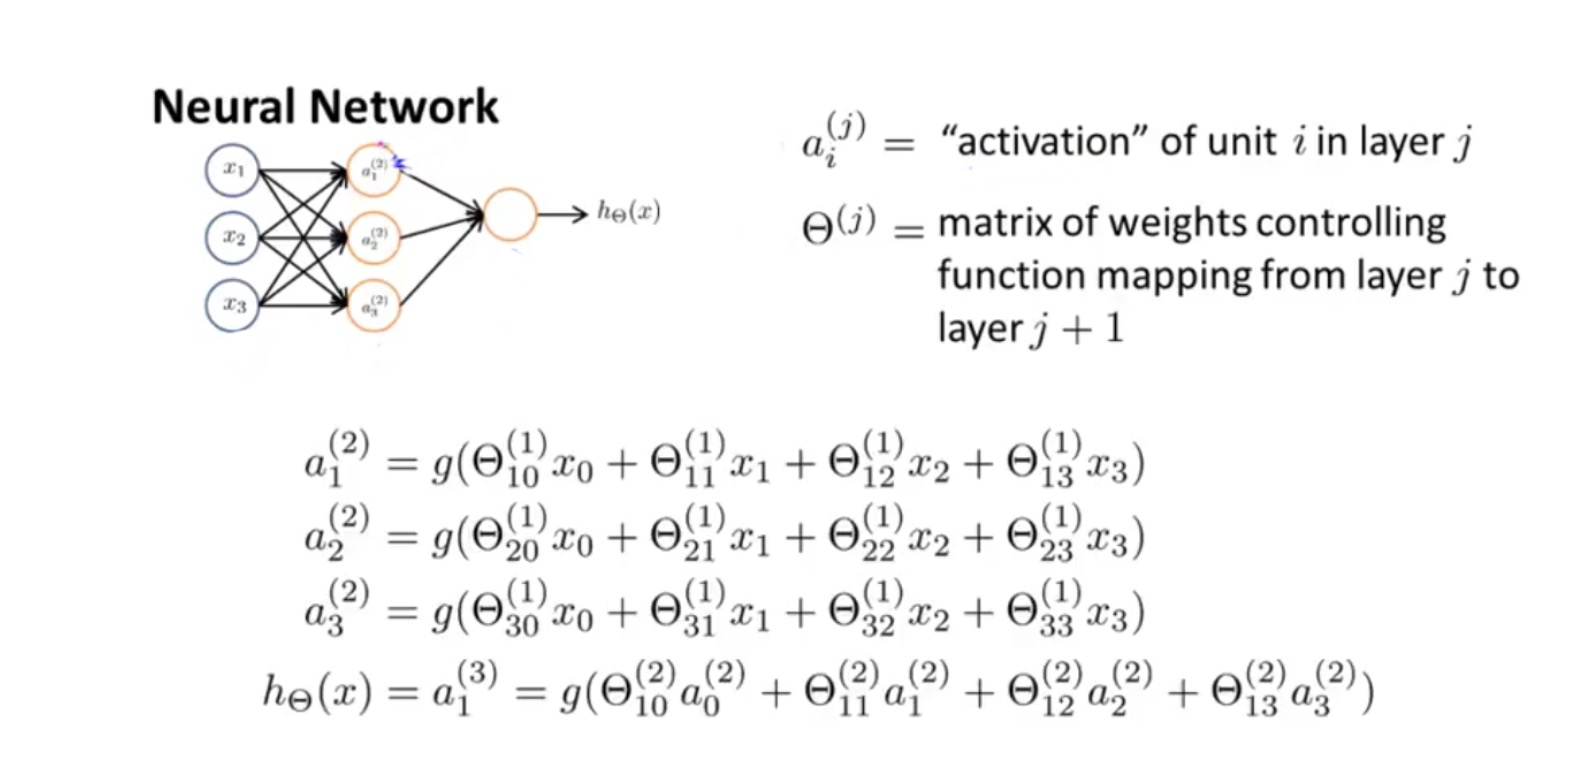
\includegraphics[width=5in]{nn.png}\\
Figure4:Neural Networks Model
\end{center}

In the \textbf{Neural Networks} model, there are 3 types of layer: input layer, hidden layer, output layer. Each layer content n nodes. After the modelization, we can compute our activation nodes by using a matrix of parameters. We apply each row of the parameters to our inputs to obtain the value for one activation node. It is used usually in  supervised learning and are creating tremendous economic value.\\

And deep learning is a Neural Network consisting of a hierarchy of layers, whereby each layer transforms the input data into more abstract representations. These series of layers, between input and output, identify the input features and create a series of new features based on the data, just as our brain. In deep learning the more layers a network has, the higher the level of features it will learn. The output layer combines all these features and makes a prediction.\\

Recent years, computer vision has also made huge strides in the last several years, mostly due to deep learning. For image applications we'll often use convolution on neural networks, often abbreviated CNN. And so for sequence data (like audios), we often use an RNN, a recurrent neural network.\\

\subsection{\textbf{Neural Networks Basics and Logistic Regression}}
\subsubsection{\textbf{Vectorization}}

In the deep learning in practice, we often train on relatively large data sets, because that's when deep learning algorithms perform better. So it's important to make sure the code run very quickly. And it will be much faster if you vectorize your code. So in this course we often try a lot to avoid the `for' loop.

Here we have one coding practice for Python photo data structure and Python basics for vectorizing computation.
\begin{center}
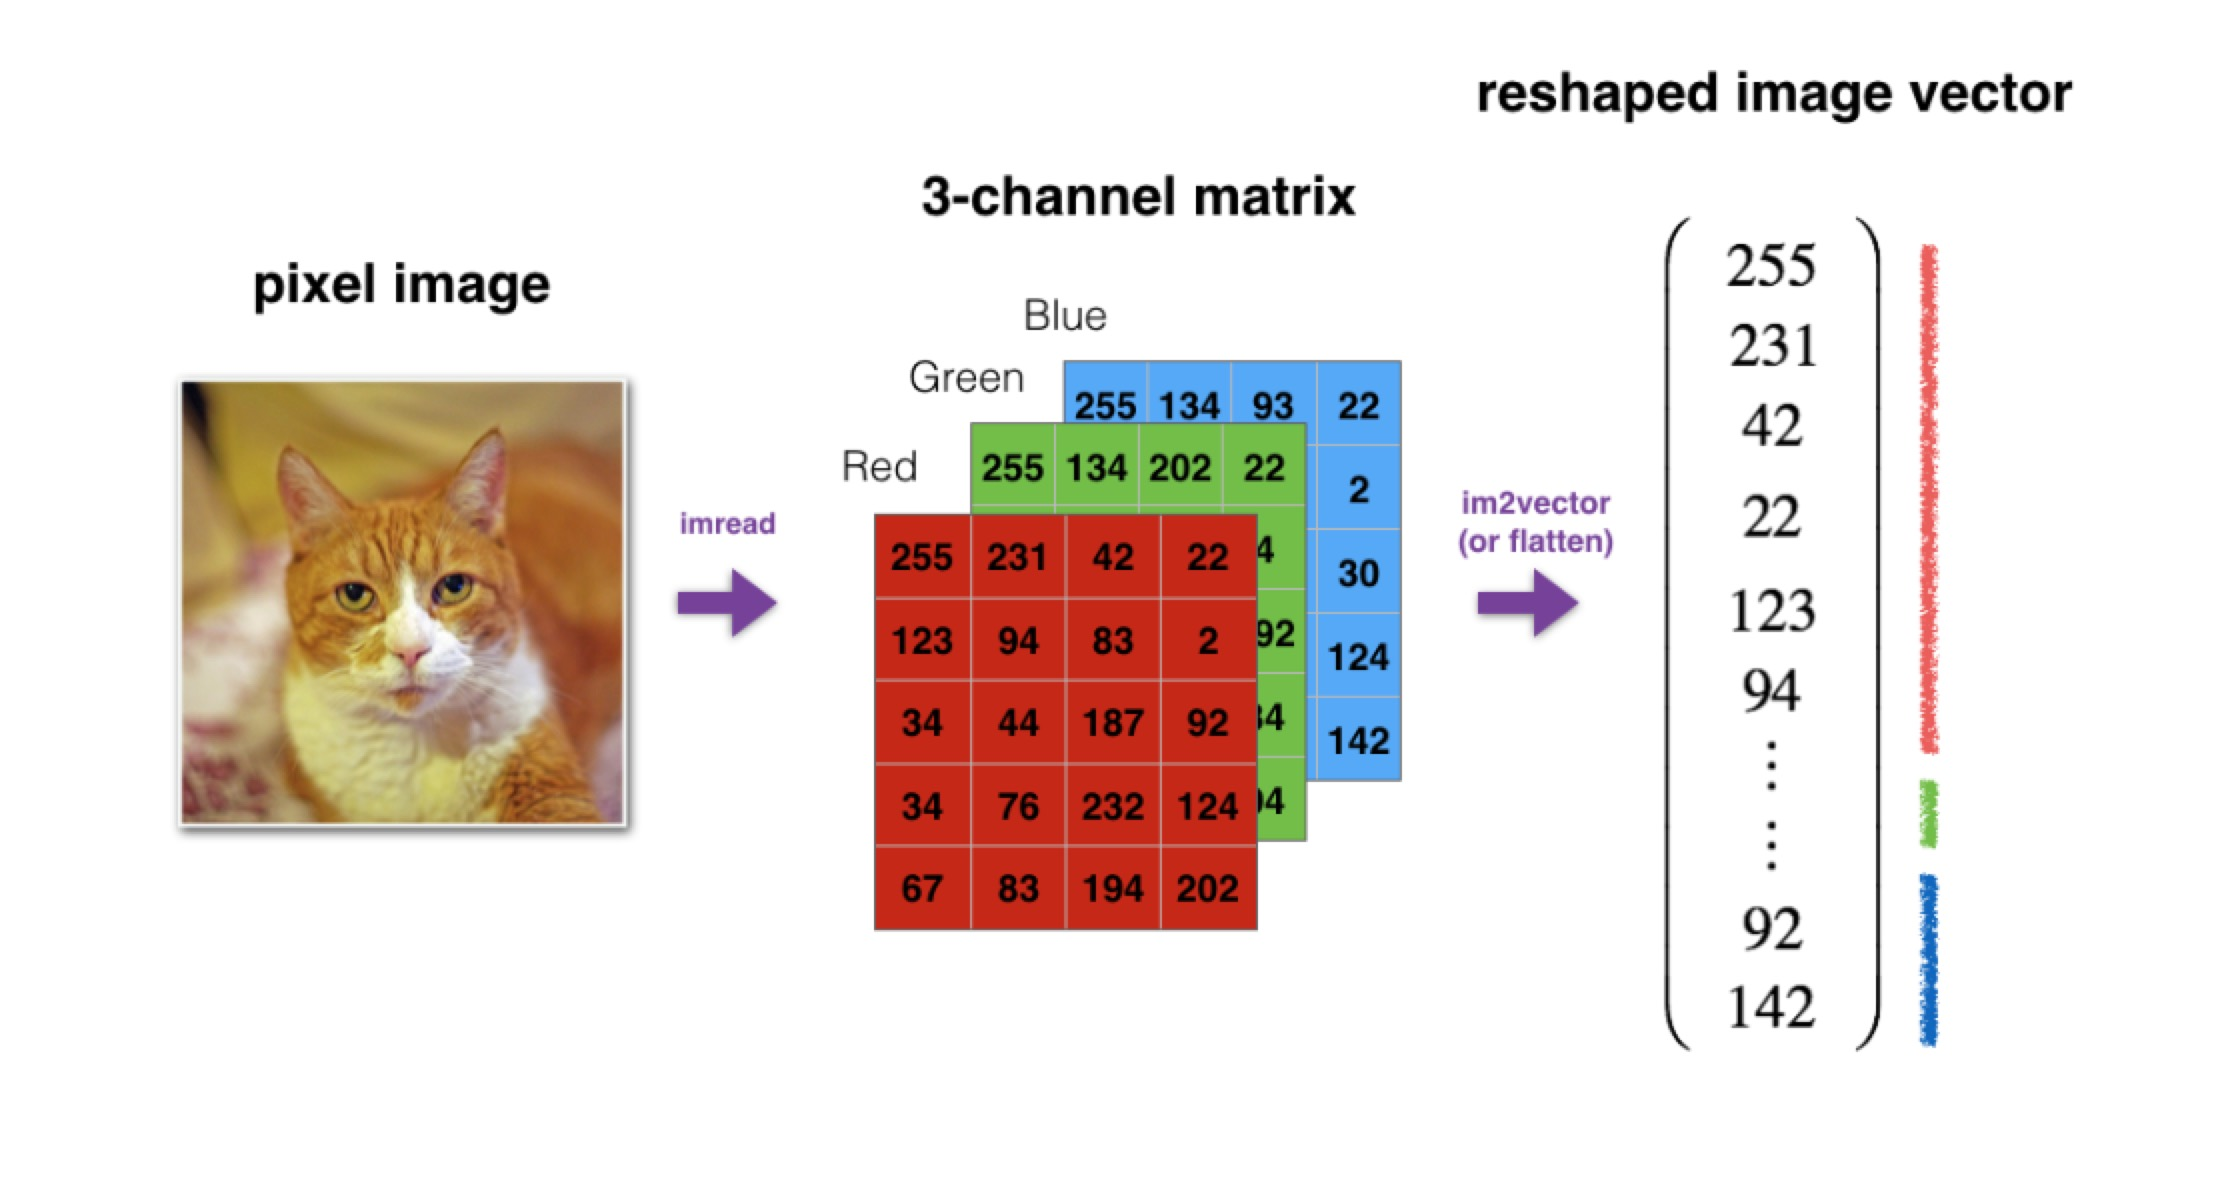
\includegraphics[width=5in]{vector.png}\\
Figure1: Photo and Vectorization
\end{center}

\subsubsection{\textbf{Logistic Regression As A Neural Network}}

In the logistic regression model, through the feature extraction, we  first select the characteristic variable x which affects the estimated variable y, and then through our training set and learning algorithm, we can get a hypothesis h. Here h can be expressed as:$$h_\theta(x)=b+w_1*x_1+w_2*x_2+...$$
And then dicide the decision boundary.
$$h_\theta(x)\ge0.5,y=1.$$
	$$h_\theta(x)<0.5,y=0.$$
Considering y equals 0 or 1, our cost function for logistic regression looks like:$$J(\theta)=-\frac{1}{m}\sum_{i=1}^m[y^{(i)}log(h_\theta(x^{(i)}))+(1-y^{(i)})log(1-h_\theta(x^{(i)}))]$$
Furthermore, with vectoration, we get:
$$Z=W^TX+b$$
$$A=\sigma(Z)\ge0.5$$
With vectorizing Logistic Regression's Gradient:
$$dZ=A-Y$$
$$dW=\frac{1}{m}XdZ^T$$
$$db=\frac{1}{m}np.sum(dZ)$$
$$W=W-\alpha (learning \ rate)\ dW$$
$$b=b-\alpha db$$
So we can finish one iteration. So here we have one project, we build a Logistic Regression, using a Neural Network mindset. And we can see that Logistic Regression is actually a very simple Neural Network.

\begin{center}
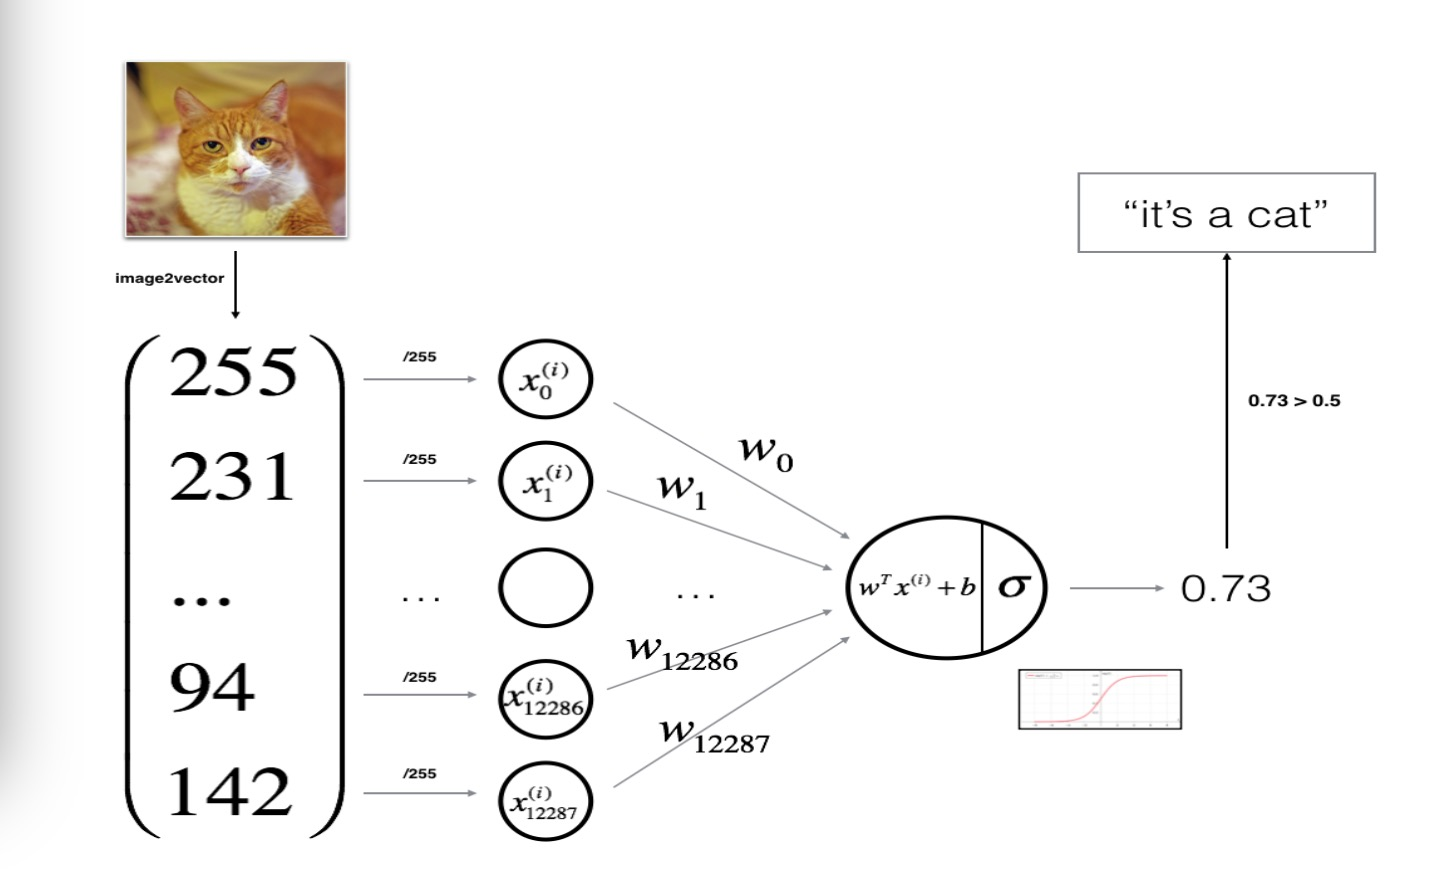
\includegraphics[width=5in]{logi.png}\\
Figure2: Mathematical expression of the logistic algorithm
\end{center}

This project is a simple image-recognition algorithm that can correctly classify pictures as cat or non-cat. Which use Logistic Regression with Neural Network minset.

\begin{center}
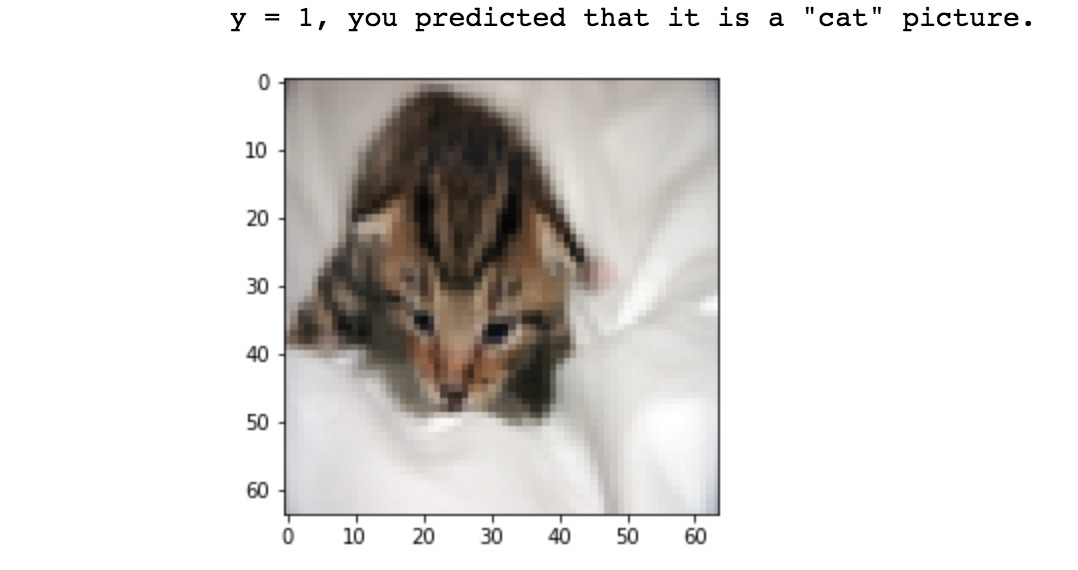
\includegraphics[width=2.5in]{reslogi.png}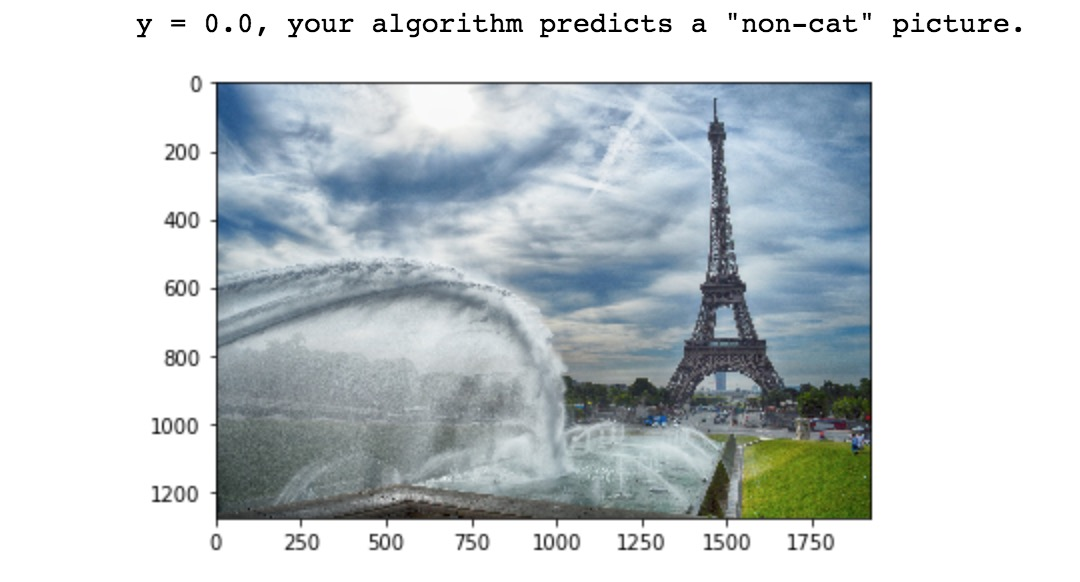
\includegraphics[width=2.5in]{reslogi2.png}\\
Figure3: Resaults for algorithm
\end{center}

\newpage

\subsection{\textbf{Shallow Neural Network}}

The third week, we study the most important algorithm for Neural Network and apply it into a shallow Neural Network.

\subsubsection{\textbf{Forward and Backpropagation}}

Neural Network with just one hidden layer is called Shallow Neural Network. With Vectorization, we compte the prediction of $y$ by Forward propagation.($\sigma( )$:activation functions)

$$a^{[1]}=\sigma (W^{[1]}x+b^{[1]})$$
$$\hat{y}=\sigma (W^{[2]}a^{[1]}+b^{[2]})$$

\textbf{``Backpropagation"} is neural-network terminology for minimizing our cost function, just like what we were doing with gradient descent in logistic regression. 
$$dz^{[2]}=\hat{y}-y$$
$$dW^{[2]}=\frac{1}{m}dz^{[2]}a^{[1]^T}$$
$$db^{[2]}=\frac{1}{m}np.sum(dz^{[2]},axis=1,keepdims=True)$$
$$dz^{[1]}=W^{[2]^T}dz^{[2]}*\sigma^{[1]'} (z^{[1]})$$
$$dW^{[1]}=\frac{1}{m}dz^{[1]}x^{^T}$$
$$db^{[1]}=\frac{1}{m}np.sum(dz^{[1]},axis=1,keepdims=True)$$

\subsubsection{\textbf{activation functions}}

When we build a neural network, we should choose what activation function to use in the hidden layers. Because if we don't have an activation function, then no matter how many layers our neural network has, all it's doing is just computing a linear activation function, which is really bad.

Here are four common activation functions, we usually use Relu for the hidden layers and Sigmoid or tanh for the outout layer.

\begin{figure}[htbp]
\centering

\subfigure[$sigmoid:\ \sigma(z)=\frac{1}{1+e^{-z}}$]{
\begin{minipage}[t]{0.3\linewidth}
\centering
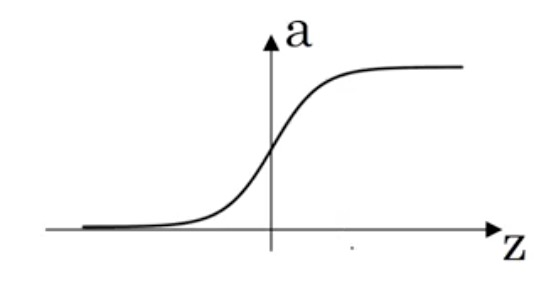
\includegraphics[width=2in]{sigmoid.png}
%\caption{fig1}
\end{minipage}%
}%
\subfigure[Tanh:$tanh(z)=\frac{e^z-e^{-z}}{e^z+e^{-z}}$]{
\begin{minipage}[t]{0.3\linewidth}
\centering
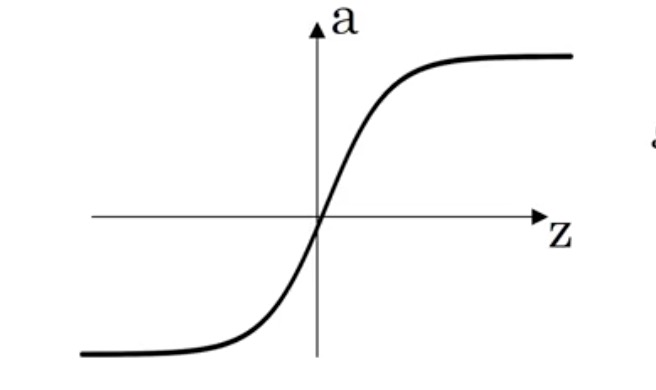
\includegraphics[width=1.6in]{tanh.png}
%\caption{fig2}
\end{minipage}%
}%
 

\subfigure[ReLU:$max(0,z)$]{
\begin{minipage}[t]{0.3\linewidth}
\centering
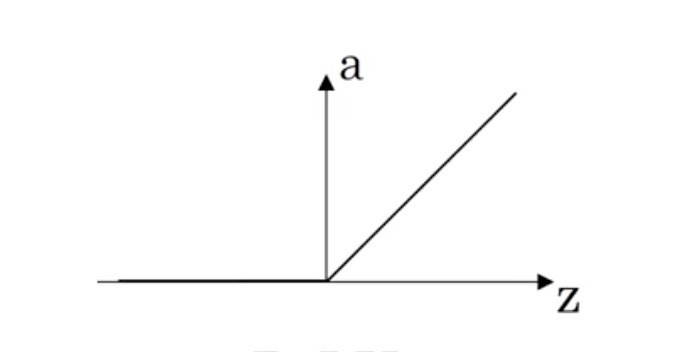
\includegraphics[width=2in]{relu.png}
%\caption{fig2}
\end{minipage}
}%
\subfigure[leakyReLU:$max(0.01z,z)$]{
\begin{minipage}[t]{0.3\linewidth}
\centering
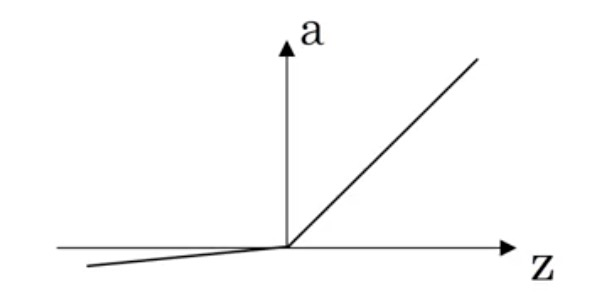
\includegraphics[width=1.9in]{lrelu.png}
%\caption{fig2}
\end{minipage}
}%

\centering
\end{figure}

\subsubsection{\textbf{Planar data classification}}

And then it's week 3 programming assignment. It's the first time to build a neural network, which has just one hidden layer. Then we compare neural network and logistic regression. We can see a big difference these two models.

\begin{center}
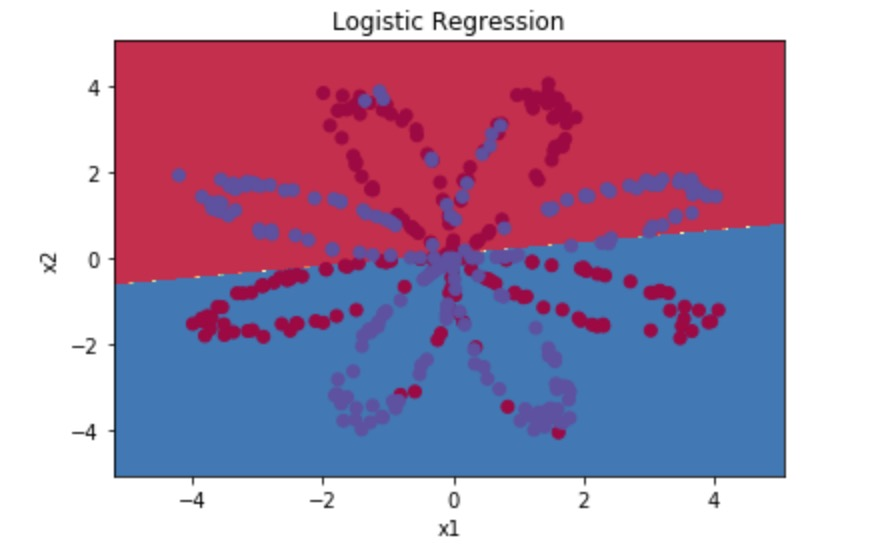
\includegraphics[width=2.5in]{resll.png}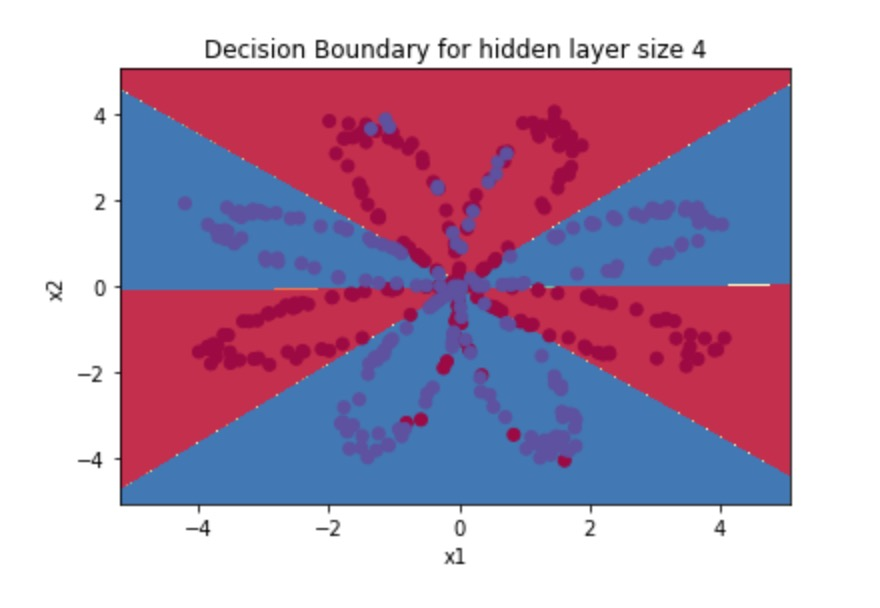
\includegraphics[width=2.5in]{resnn.png}\\
Figure4: Resaults for data classification
\end{center}

\subsection{\textbf{Deep Neural Networks}}

For implementing the Deep Neural Net with $L$ layers, we need to use one activation function that replicates the previous layer L−1  times( usually RELU activation function), then follows with another one activation function(usually SIGMOID).

\begin{center}
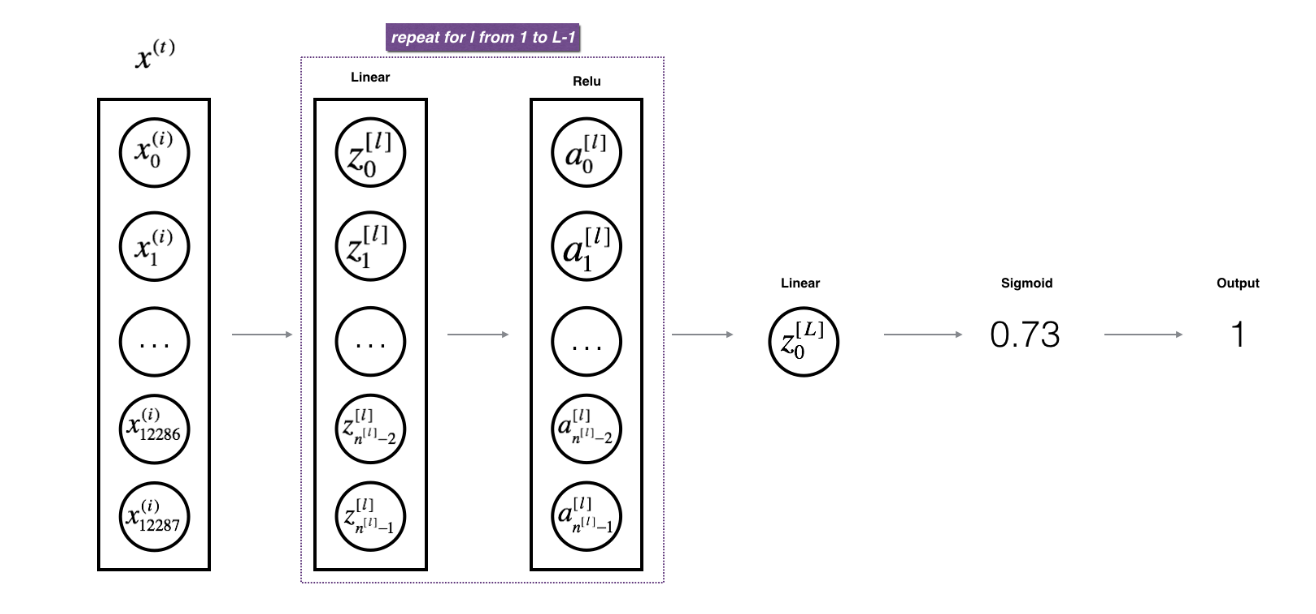
\includegraphics[width=5in]{NNL.png}\\
Figure5: L-layers Neural Net model
\end{center}

So for the forward propagation, we use the equations bellow:
$$A^{[l]}=\sigma(Z^{[l]})=\sigma(W^{[l]}A^{[l-1]}+b^{[l]})$$
And the cost function become to:
$$-\frac{1}{m}\sum_{i=1}^{m}(y^{(i)}log(a^{[L](i)})+(1-y^{(i)})log(1-a^{[L](i)}))$$
So for the back propagation, we need to update the parameters from $L$ layer to the first layer:
$$dW^{[l]}=\frac{1}{m}dZ^{[l]}A^{[l-1]T}$$
$$db^{[l]}=\frac{1}{m}\sum_{i=1}^mdZ^{[l](i)}$$
$$dA^{[l-1]}=W^{[l]T}dZ^{[l]}$$

\begin{center}
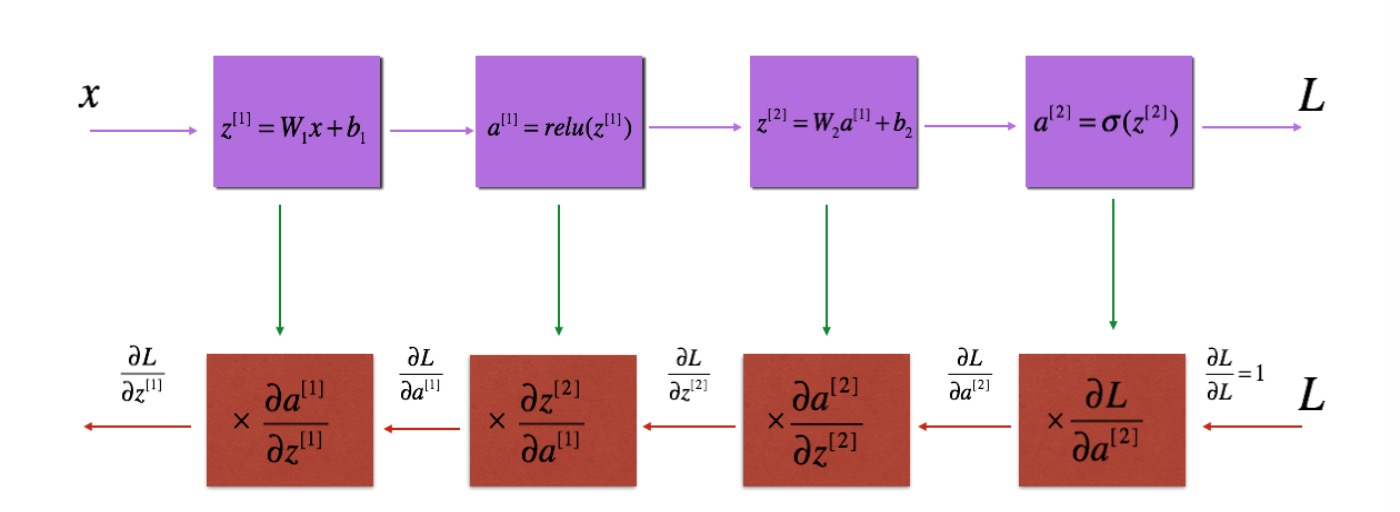
\includegraphics[width=5in]{LNNfb.png}\\
Figure6:  Forward and Backward propagation for L-layers Neural Net model
\end{center}

Then we do the most important project of this course, we build a 4-layer neural networks with 12288, 20, 7 and 5 dimensions, and train it to the task of cat vs non-cat classification. And for the activation functions, we use ReLU function for the first 3 layer, and sigmoid function for the last layer.

\begin{center}
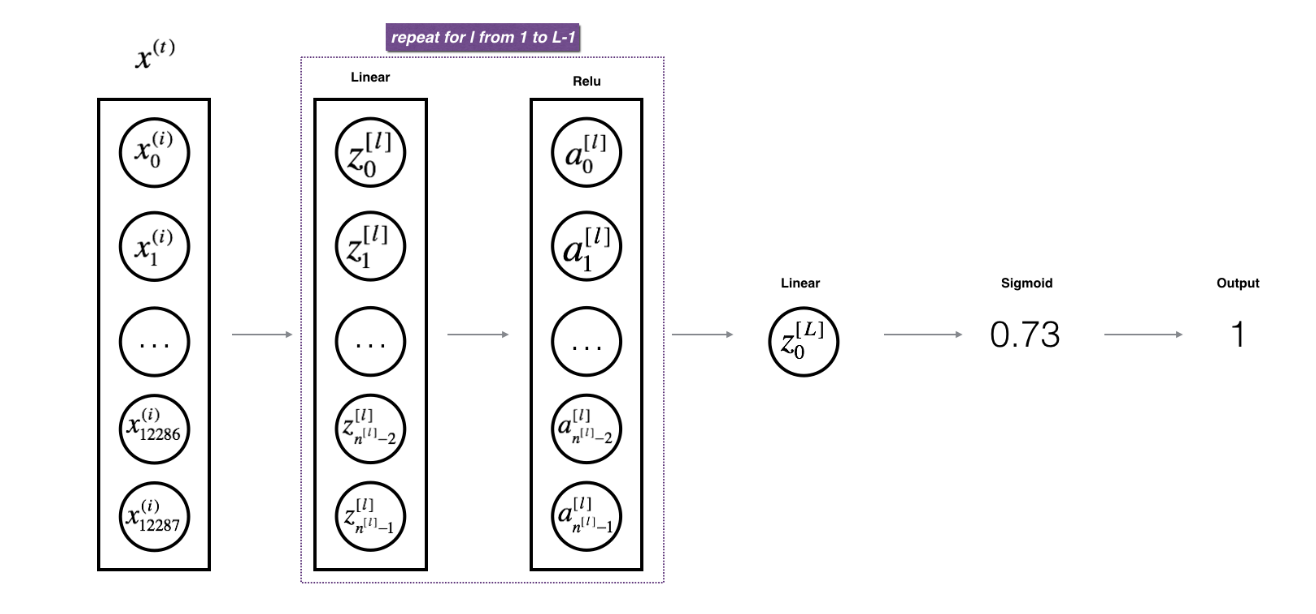
\includegraphics[width=5in]{NNL.png}\\
Figure7: Result of cat vs non-cat classification
\end{center}

To compare with the result of the logistic regression model, the accuracy increase from 68\% to 80\%.

\newpage

\section{Improving Deep Neural Networks}

This part is important for getting deep learning to work better. This second course of the Deep Learning Specialization include initialization, L2 and dropout regularization, Batch normalization, and some optimization algorithms, such as mini-batch gradient descent, Momentum, RMSprop and Adam. I just finish two weaks of this course, there are the main points below.

\subsection{Initialization}

Training a neural network requires specifying an initial value of the weights. A well chosen initialization method will help learning to speed up the convergence of gradient descent and increase the odds of gradient descent converging to a lower training  error.

With the different ways to initialize the parameters, we can see that a big difference:

\begin{center}
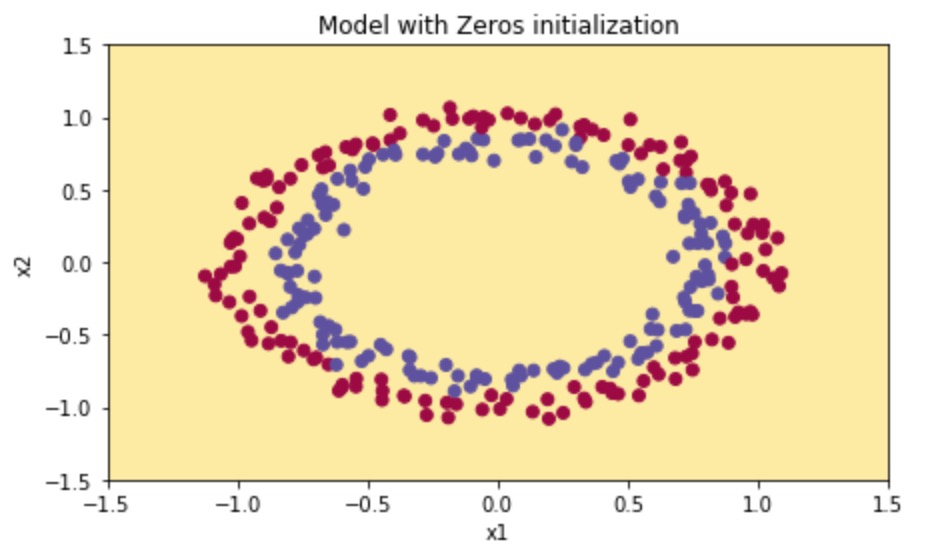
\includegraphics[width=1.8in]{zero.png}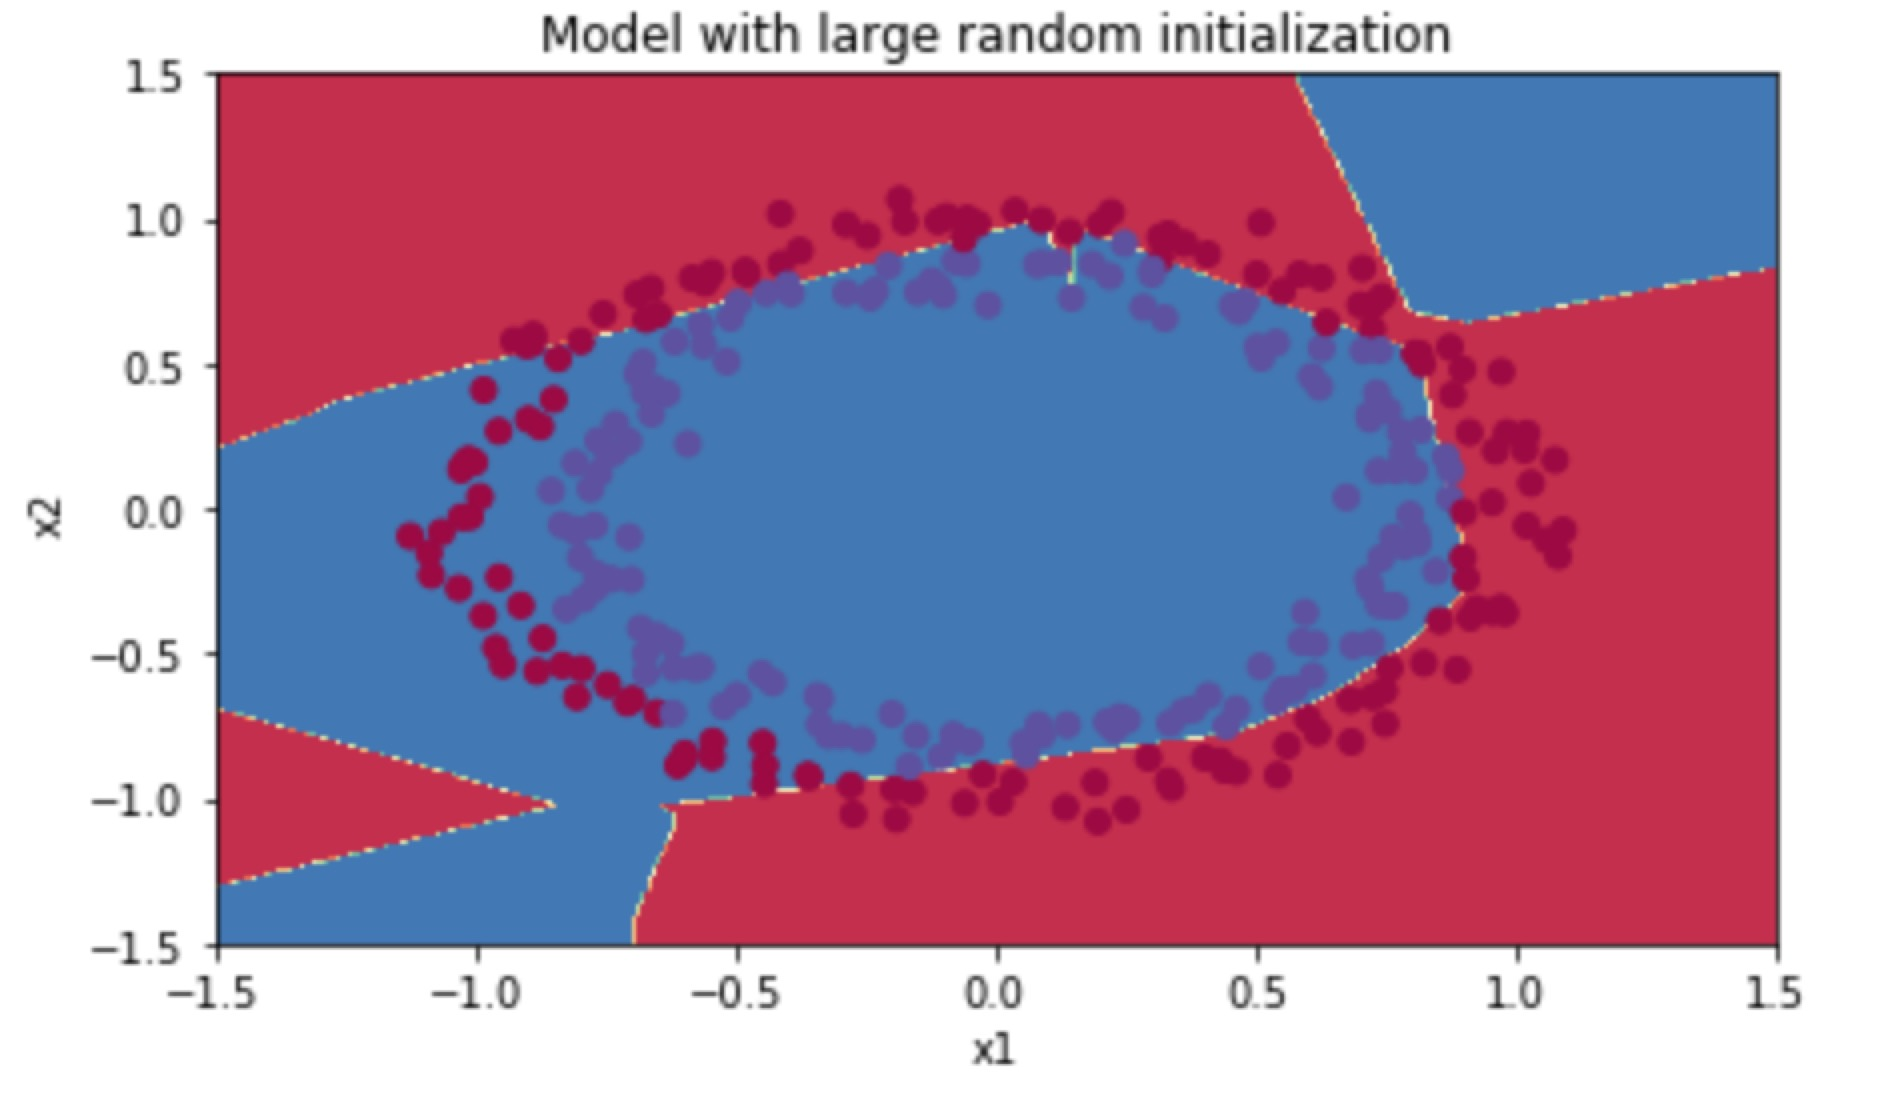
\includegraphics[width=1.8in]{rand.png}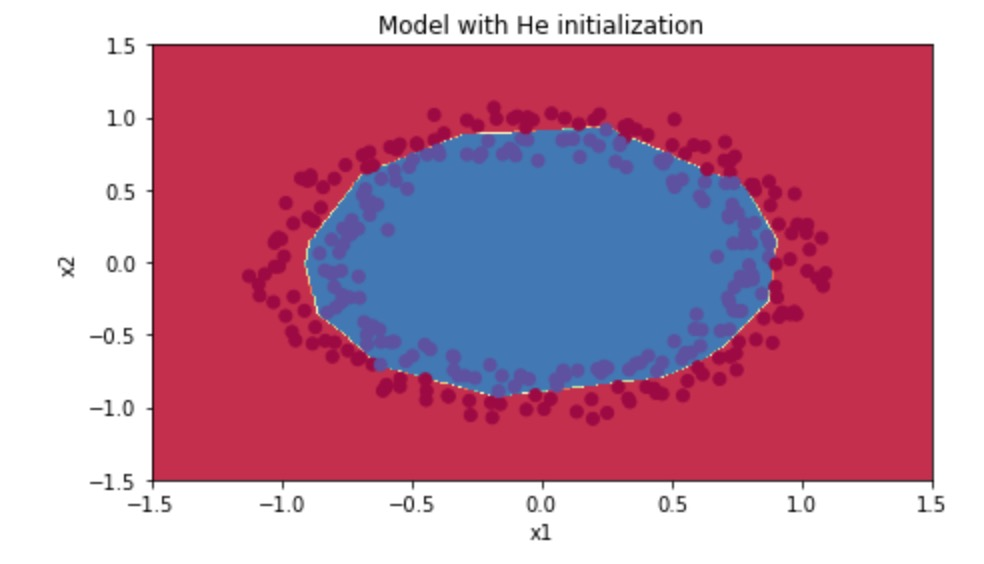
\includegraphics[width=1.8in]{he.png}\\
Figure8: Various Initialization
\end{center}

For this case, if we initialize parameters as 0, the model we get will be very bad. With random initialization, the result is better. And with He method(Random initialization multiply with $\sqrt{\frac{2}{dimension\ of\ previous\ layer}}$), we have the best model.

\subsection{Regularization}

Sometimes, our model could get the overfitting issus, which means the model has a low training error but perform bad for the test dataset. Here we learn different regularization methods include L2 and dropout regularizatin. 

L2 adds “squared magnitude” of coefficient as penalty term to the cost function. 
$$Cost\ function = Cost\ function+ \frac{1}{2} \frac{\lambda}{m}W^2$$
And we also need to implement the changes in backward propagation to take into account regularization.
$$dW=dW+\frac{d}{dW}(\frac{1}{2} \frac{\lambda}{m}W^2)=dW+\frac{\lambda}{m}W$$

Finally, dropout is a widely used regularization technique that is specific to deep learning. It randomly shuts down some neurons in each iteration. So for each neuron unit, it will become less sensitive to the activation. So it used to fix the overfitting problem.

\begin{center}
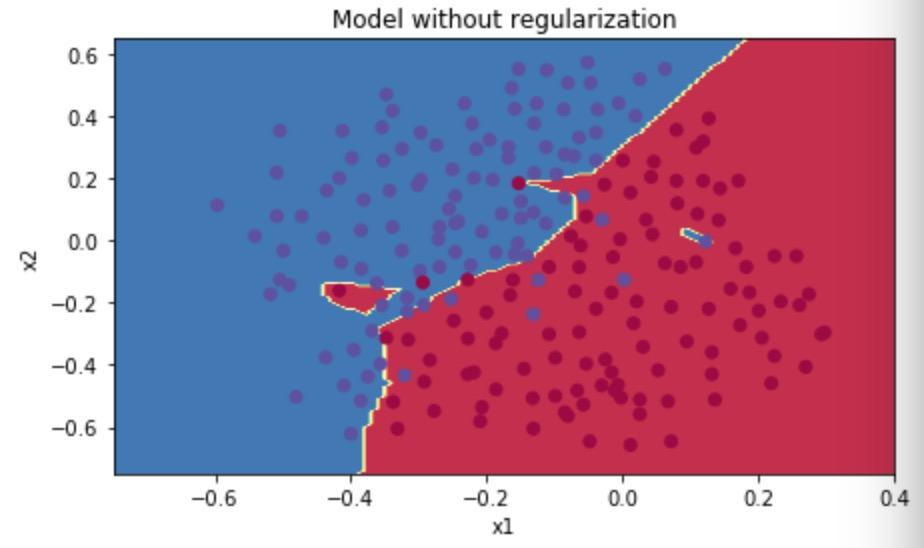
\includegraphics[width=1.8in]{nore.png}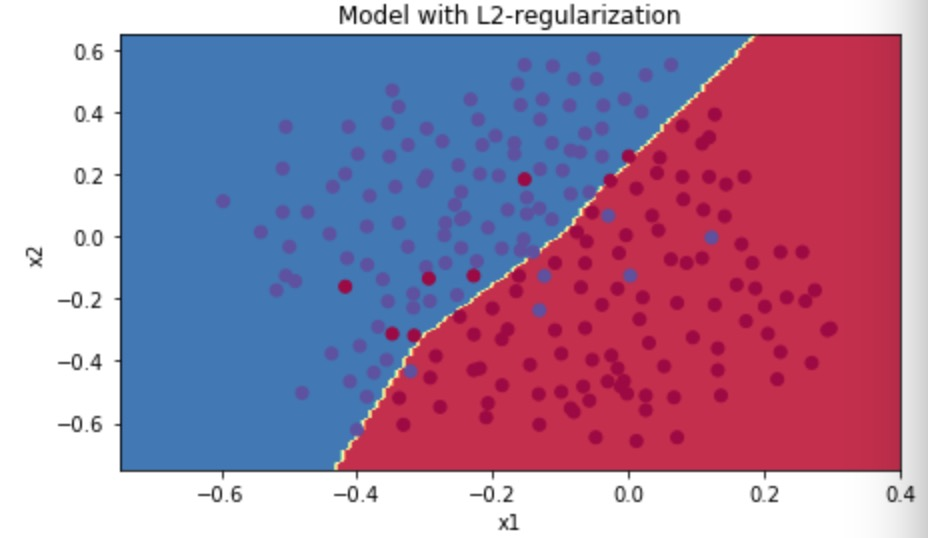
\includegraphics[width=1.8in]{l2.png}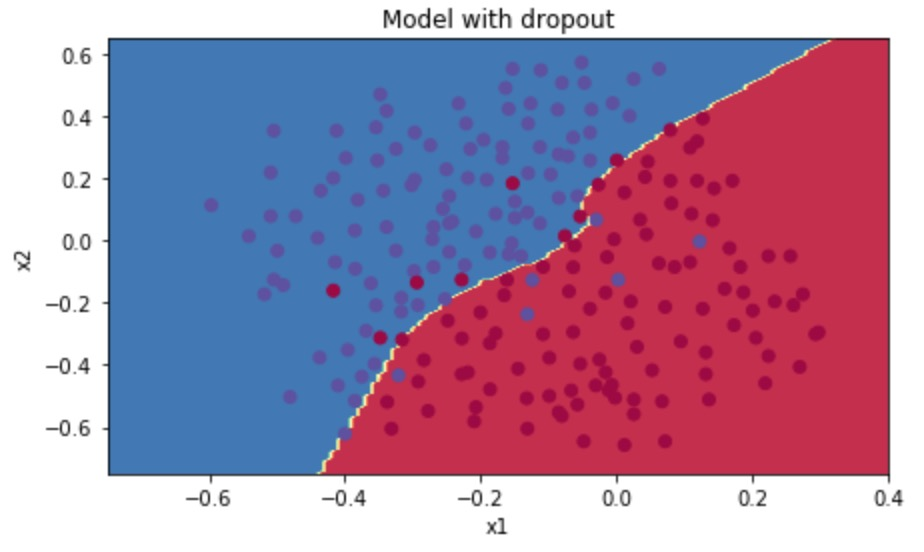
\includegraphics[width=1.8in]{drop.png}\\
Figure8: Various Initialization
\end{center}

\subsection{Optimization}

\textbf{Mini-batch gradient descent}\\
Nowadays, big data is a very porpular domain, but Deep Learning does not work best in a this regime. When we neural networks on a huge data set we find that it's really slow. But with mini-batch gradient descent algorithm, we can speed up the efficiency.

The main idea is that split up your training set into smaller sets which are called mini-batches. For each mini-batche, the model could complete once learning iteration. So for one epoch(Traverse once dataset), it can take 5,000 gradient descent steps rather than 1  gradient descent steps in general batche gradient descent. So when we have a huge training set, mini-batch gradient descent runs much faster than batch gradient descent.\\

\textbf{Momentum algorithm}\\
Momentum compute an exponentially weighted average of the gradients, and then use that gradient to update the weights.
$$v_{dW}=\beta v_{dW} + (1-\beta)dW$$
$$v_{db}=\beta v_{db}+ (1-\beta )db$$
$$W=W-\alpha v_{dW}, b = b - \alpha v_{db}$$
So when we do the gradient descend, it will gain momentum. So it could speed up learning for some parameters, at the same time slow down some others. So we can reach the convergence point quickly.\\

\textbf{RMSprop}\\
RMSprop stands for root mean square prop. It's idea is similar with Momentum algorithm except it adds an exponentially weighted average of the squares of the derivatives.
$$S_{dW}=\beta S_{dW} + (1-\beta)dW^2$$
$$S_{db}=\beta S_{db}+ (1-\beta )db^2$$
$$W=W-\alpha \frac{dW}{\sqrt{S_{dW}}}, b = b - \alpha \frac{db}{\sqrt{S_{db}}}$$\\

\textbf{Adam optimization algorithm}\\
Adam optimization algorithm is basically taking momentum and RMSprop and putting them together. Adam is one of those rare algorithms that has really stood up, and has been shown to work well across a wide range of deep learning architectures.
$$v_{dW}=\beta v_{dW} + (1-\beta)dW,\ v_{db}=\beta v_{db}+ (1-\beta )db$$
$$S_{dW}=\beta S_{dW} + (1-\beta)dW^2,\ S_{db}=\beta S_{db}+ (1-\beta )db^2$$
$$W=W-\alpha \frac{v_{dW}}{\sqrt{S_{dW}}+\epsilon}, b = b - \alpha \frac{v_{db}}{\sqrt{S_{db}}+\epsilon}$$

\subsection{Tool and Language}
\textbf{Jupiter iPython}\\
This course use Jupiter iPython notebook for the programming exercises, it has the interactive command shell nature which is very useful for learning quickly. We use the package `numpy' and `math' for computing, `scipy.io' and `sklearn' for the datas, and `matplotlib.pyplot' for show the result.

\newpage
\section{Conclusion}
After a period of study, I learned about the most effective deep learning techniques, and gain practice implementing them and getting them to work for myself. From this course, I find that there are still many interesting things during this domain, I will keep learning and make myself to be a better data scientist. To conclusion, I benefit a lot from this course.

\section{Appendix}

Course:\href{https://www.coursera.org/specializations/deep-learning}{https://www.coursera.org/specializations/deep-learning} \\
After 6 weeks studying, I passed this course. My final resault is 96/100.
\begin{center}
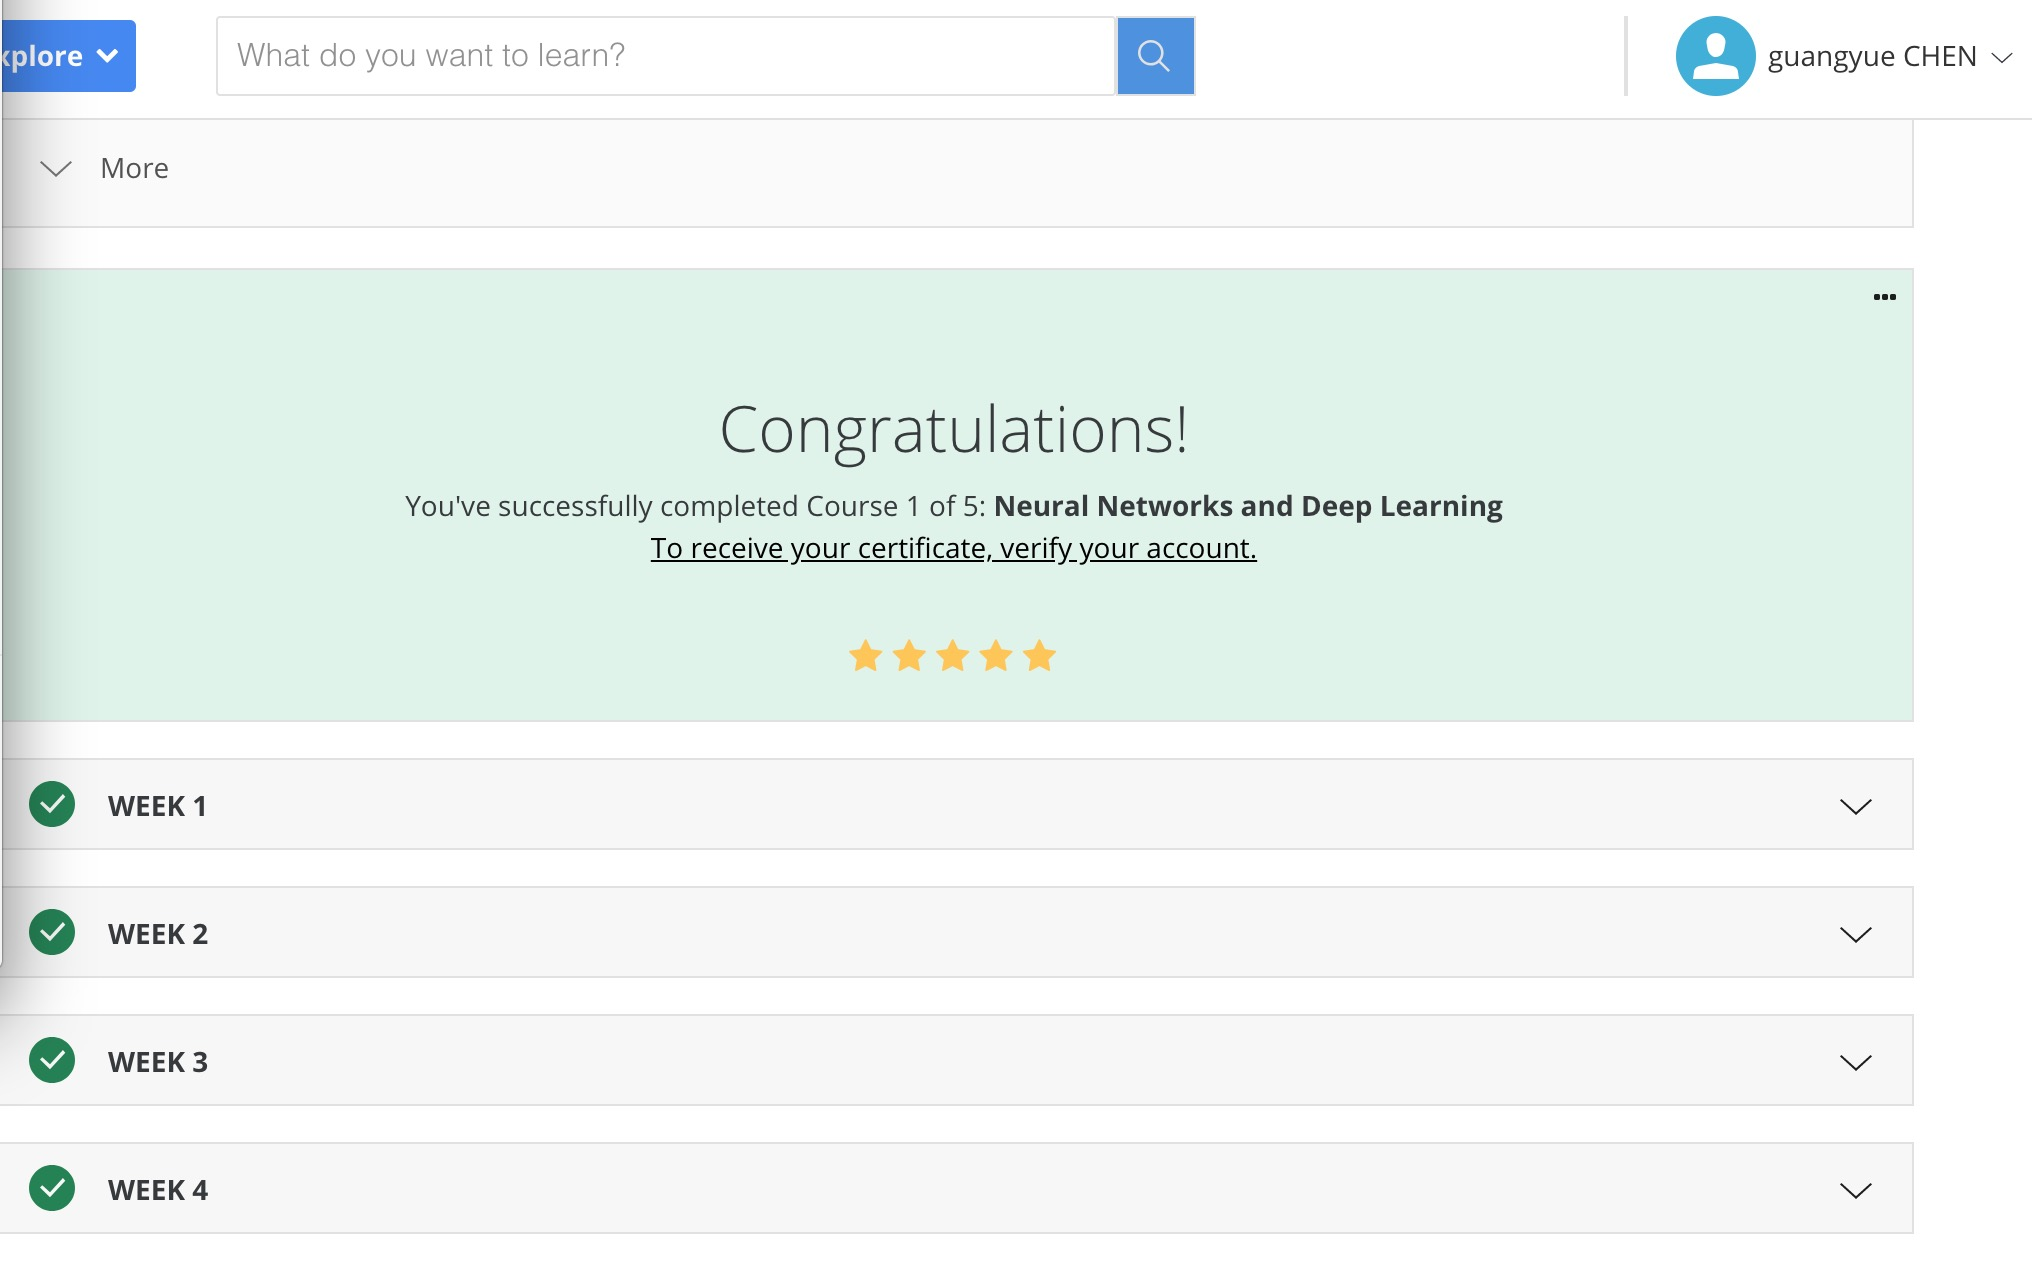
\includegraphics[width=5in]{res1.jpeg}
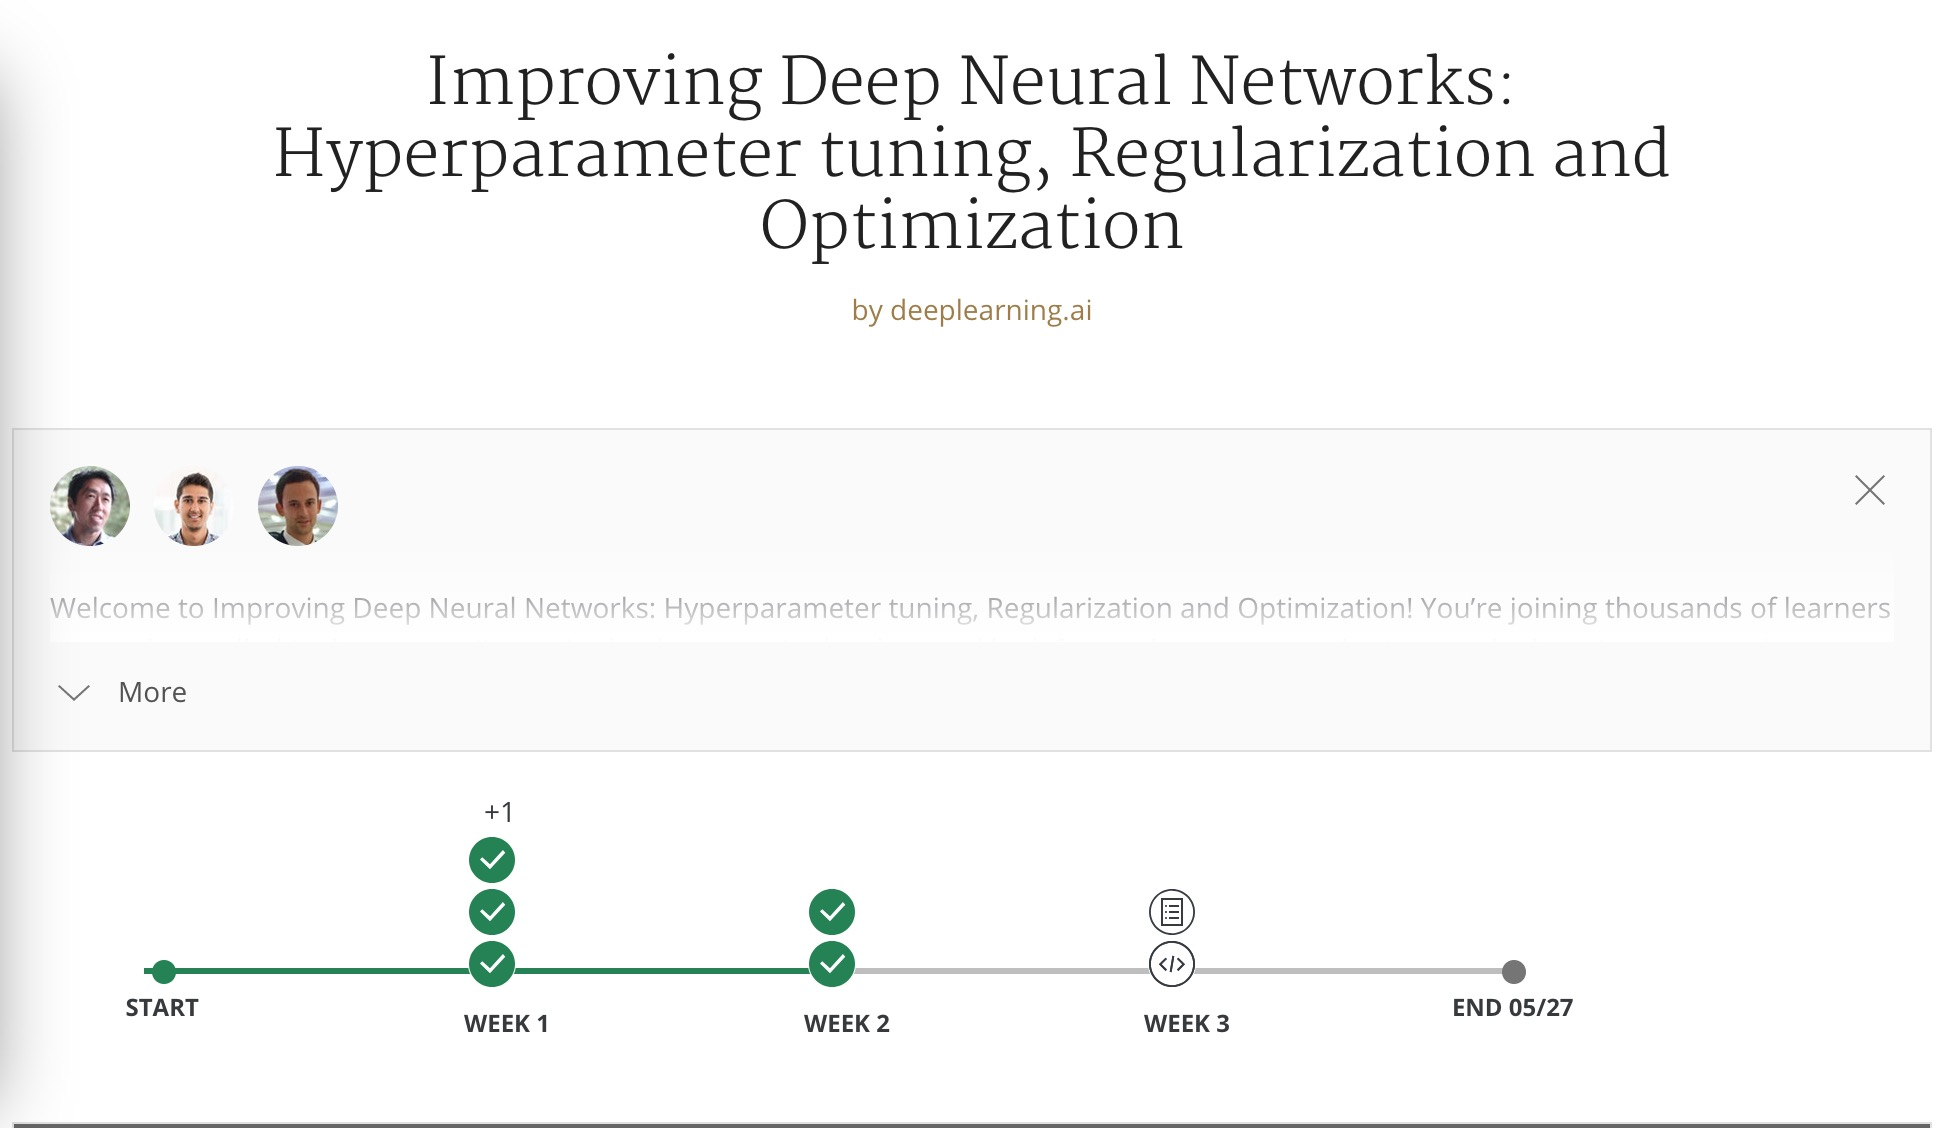
\includegraphics[width=5in]{res2.jpeg}
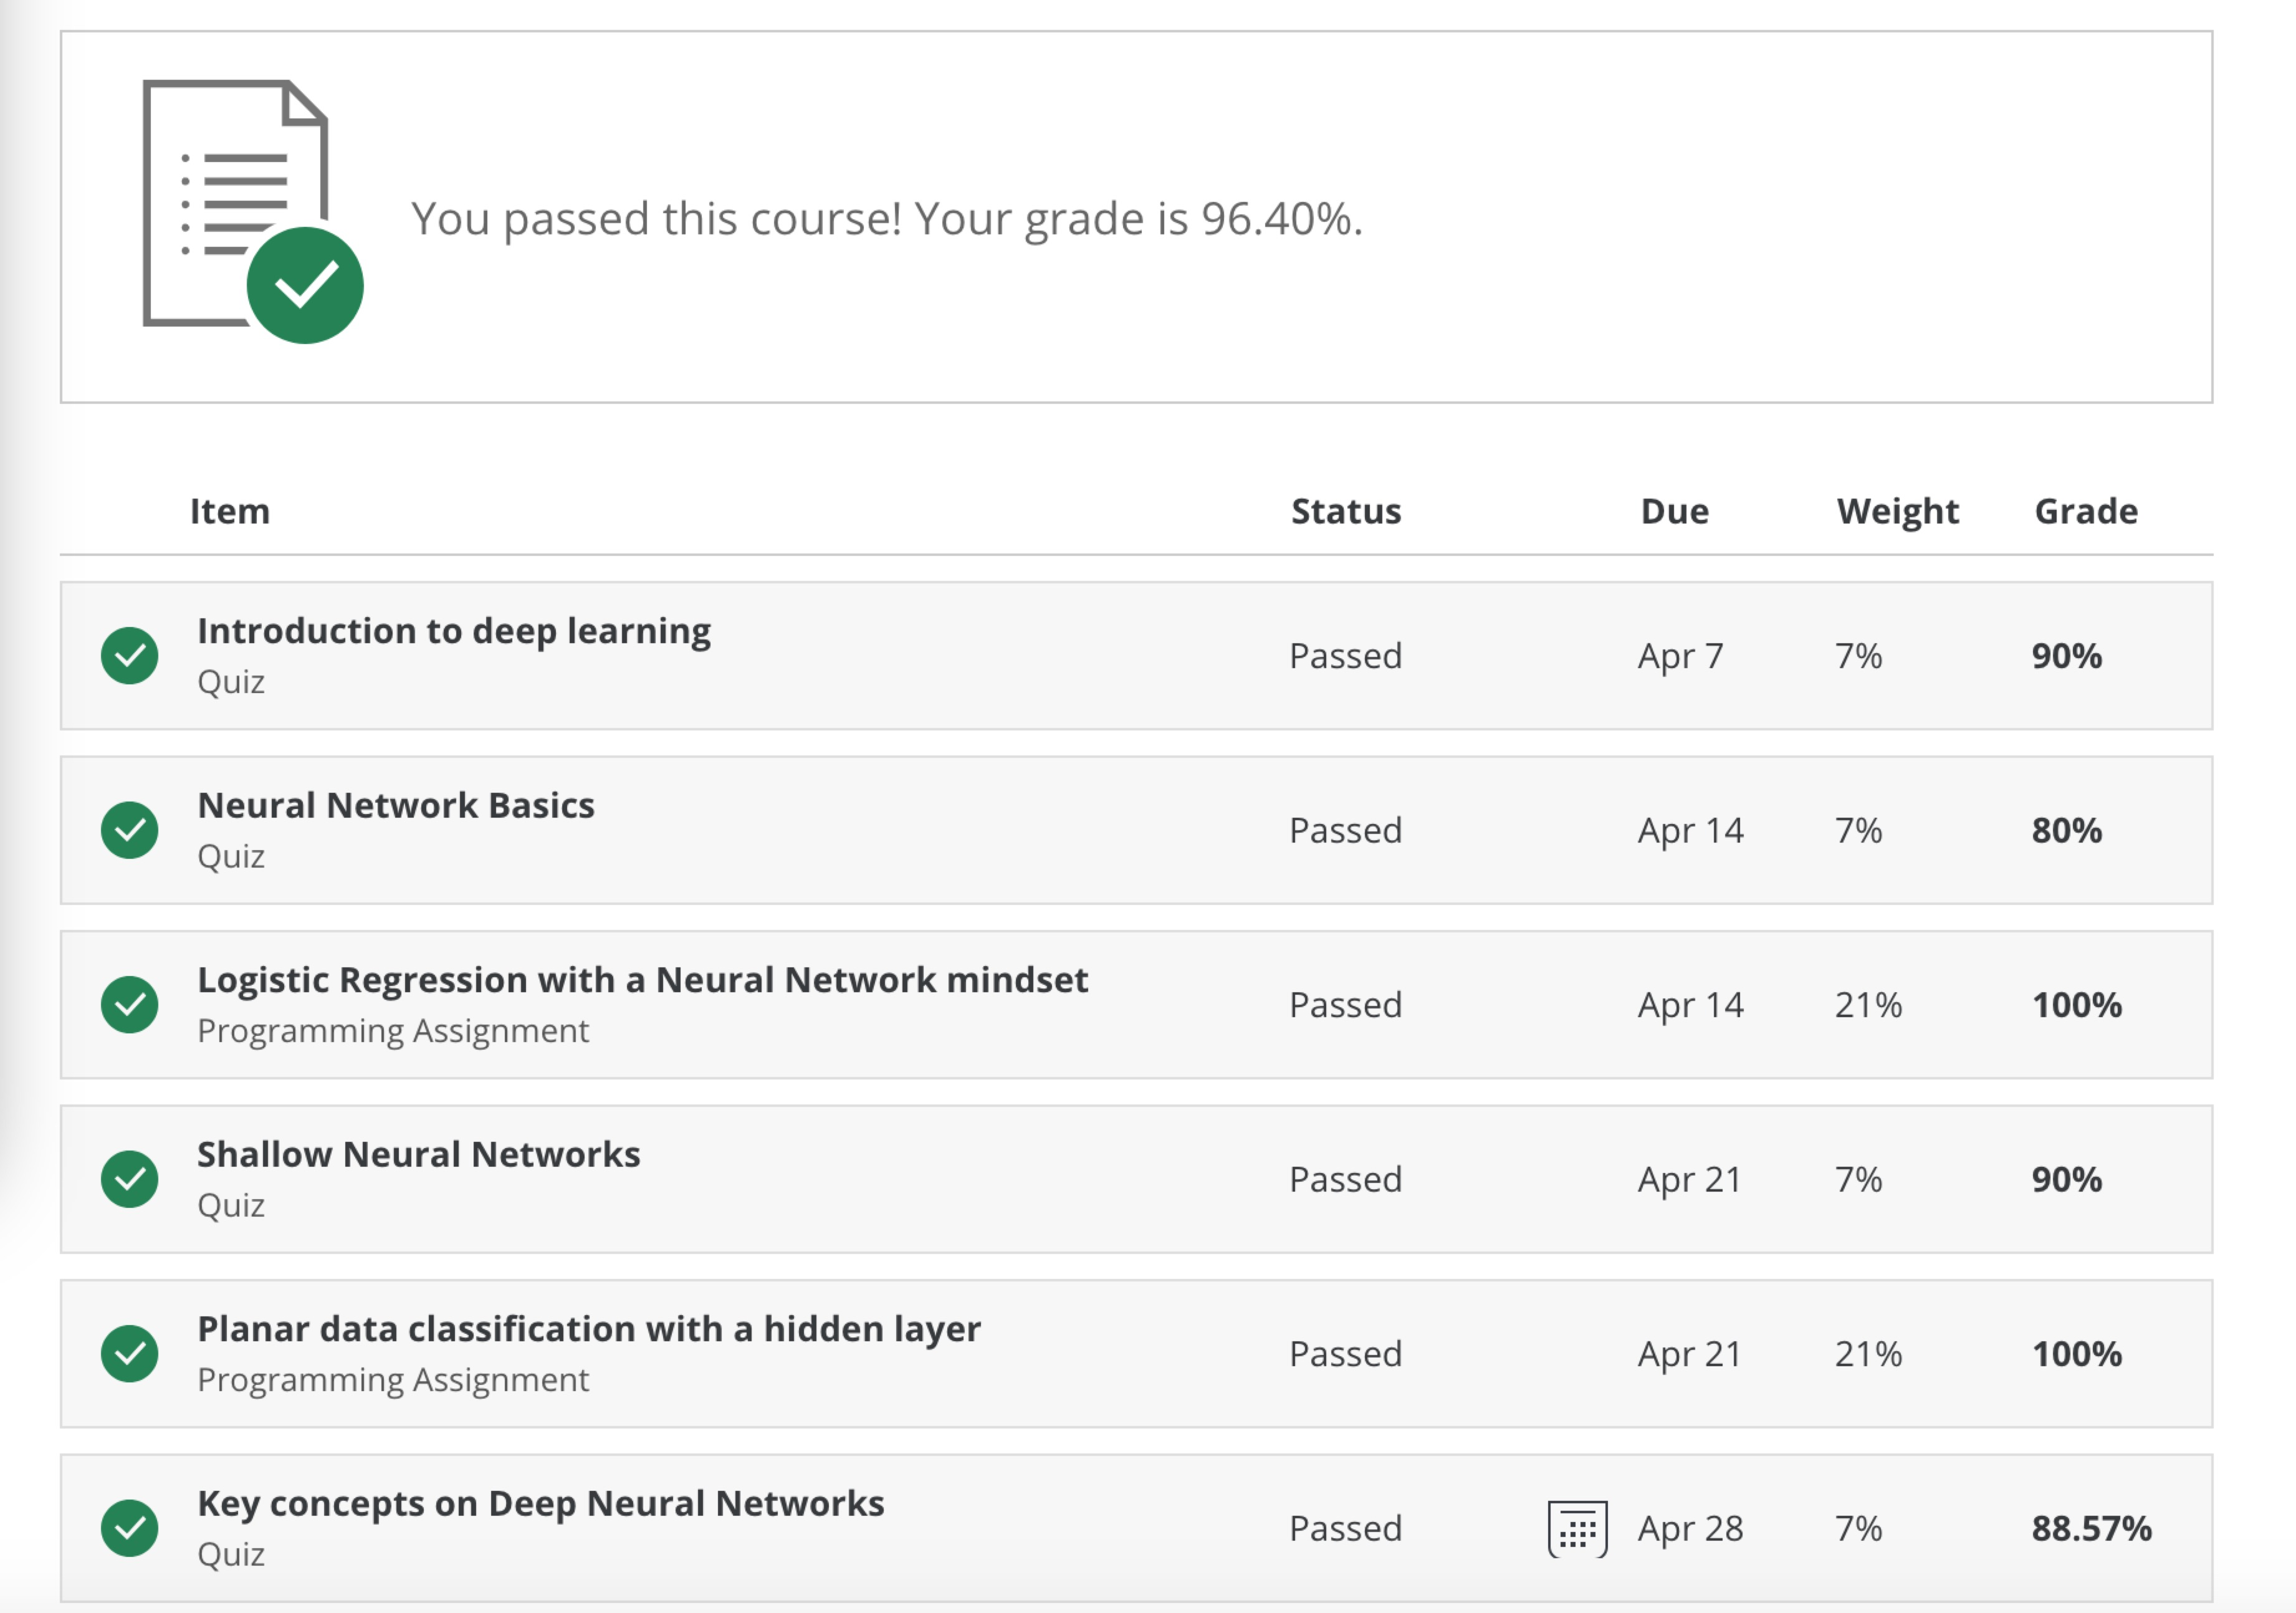
\includegraphics[width=5in]{res3.jpeg}
\end{center}
\end{document}